\section{Theory}\label{sec:Theory}

\subsection{Ordinary Least Squares}\label{subsec:OLS}

Let \(Y\) be a stochastic variable denoting the observed response of some
phenomena, with \(X_{i}\) being the predictors assumed to describe and predict
it by the relation:
\begin{equation*}
  Y = f(X) + \varepsilon
\end{equation*}
where \(f\) is the true relationship and \(\varepsilon\) the random error
with \(E(\varepsilon) = 0\) and \(Var(\varepsilon) = \sigma^{2}\).

\textit{Regression} is the process of approximating \(f\)
by some model. The simplest form is linear regression where a affine model is
used, written:

\begin{equation*}
  \hat{Y} = \hat\beta_{0} + \sum_{j=0}^{p}X_{j}\hat\beta_{j}
\end{equation*}

or using matrix notation:

\begin{equation*}
  \hat{Y} = X^{T}\hat\beta
\end{equation*}

The \(X\) matrix is called the \textit{design matrix}, whose first column is
constant 1s to account for the bias term \(\hat\beta_{0}\).

Fitting the linear model to the observed data is often done by minimizing the
residual sum of squares:

\begin{equation*}
  RSS(\beta) = \sum_{i=1}^{N} \left( y_{i} - x_{i}^{T}\beta \right)^{2}
\end{equation*}

or in matrix notation:

\begin{equation*}
  RSS(\beta) = (\vb{y} - \vb{X}\beta)^{T}(\vb{y} - \vb{X}\beta)
\end{equation*}

Differentiating with respect to \(\beta\) gives the normal equations, whose
solution gives \(\beta\) as:

\begin{equation*}
  \hat\beta = \left(\vb{X}^{T}\vb{X}\right)^{-1}\vb{X}\vb{y}
\end{equation*}

From which the prediction \(\vb{\hat y}\) can be found as:

\begin{equation*}
  \vb{\hat y} = \vb{X}\hat\beta = \vb{X}\left(\vb{X}^{T}\vb{X}\right)^{-1}\vb{X}\vb{y} = \vb{H}\vb{y}
\end{equation*}

The \textit{hat matrix} or \textit{projection matrix}

\begin{equation*}
  \vb{H} =\vb{X}\left(\vb{X}^{T}\vb{X}\right)^{-1}\vb{X} 
\end{equation*}

is called so as it
projects \(\vb{y}\) onto the subspace spanned by \(\vb{X}_{i}\)
often useful in further analysis, as we'll see later.

The variance of the OLS estimate is:

\begin{equation*}
  \text{Var}(\hat\beta) = \left( \vb{X}^{T}\vb{X} \right)^{-1}\sigma^{2}
\end{equation*}
where \(\sigma\) is often estimated by the maximum likelihood estimator (MLE)

\begin{equation*}
  \hat\sigma^{2} = \frac{1}{N-p-1}\sum_{i=1}^{N}\left( y_{i} - \hat y_{i} \right)^{2}
\end{equation*}

The estimator is then distributed as:

\begin{equation*}
\hat\beta \sim N\left( \beta, \left( \vb{X}^{T}\vb{X} \right)^{-1}\sigma^{2} \right)
\end{equation*}

The \(Z\)-score used for hypothesis testing can be found CITE to be

\begin{equation*}
  z_{i} = \frac{\hat\beta_{i}}{\hat\sigma\sqrt{v_{i}}}
\end{equation*}
where \(v_{i}\) is the \(\text{i}^{\text{th}}\) diagonal element of \(\left( \vb{X}^{T}\vb{X} \right)^{-1}\).
The corresponding confidence interval is therefore:

\begin{equation*}
  \left( \hat\beta_{i} - z^{1-\alpha}\sqrt{v_{i}}\hat\sigma,  \hat\beta_{i} + z^{1-\alpha}\sqrt{v_{i}}\hat\sigma\right)
\end{equation*}

An interpretation of minimizing the \(RSS\) is that the area spanned by the
error at each observation is the smallest possible, as illustrated by~\cref{fig:lq}.
\begin{figure}[]
  \centering
  \showthe\columnwidth
  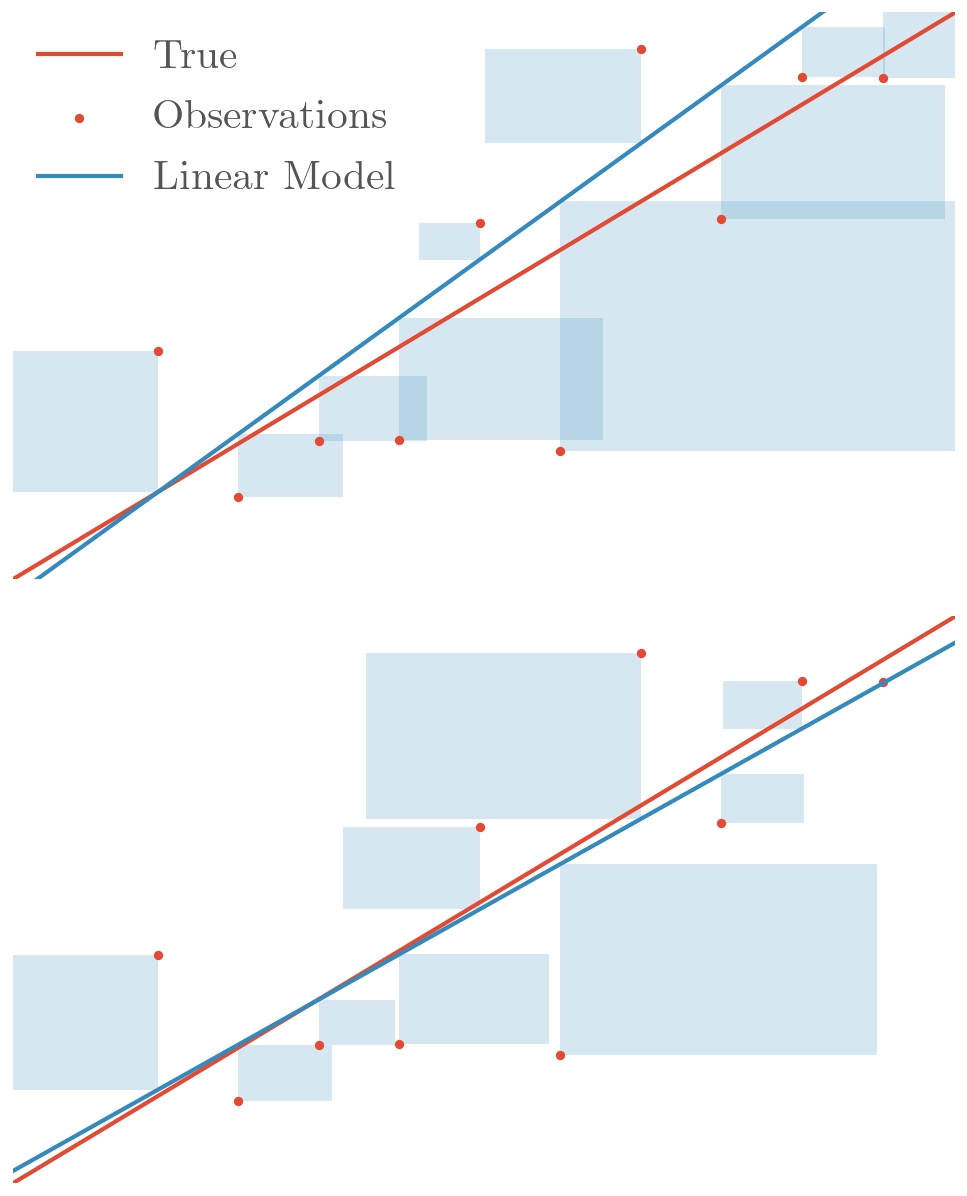
\includegraphics[]{figures/leastsquares.png}
  \caption{\label{fig:lq} Illustration of the principle of least squares. A
    sample of points are shown in both plots which are drawn from the true
    relationship (orange line) with some random noise. A linear model is
    guessed at, resulting in the blue line in the upper plot. The square error at
    each both is drawn as blue rectangles, the sum of their areas being RSS. By
    minimizing this area we obtain the OLS estimate, shown in the lower plot.}
\end{figure}

For assessing the goodness of fit, the \textit{coefficient of determination}
\(R^{2}\) is often used. It is the ratio of explained variance to total variance:

\begin{equation*}
  R^{2} = 1 - \frac{RSS}{TSS} = \frac{\sum \left(\hat y_{i} - \bar{y} \right)^{2}}{\sum\left(y_{i} - \bar y \right)^{2}}
\end{equation*}

However, in practice the equivalent measure \textit{mean square error} is used instead.

The degrees of freedom describes the ability of a model to explain the variance
in a data set. For a \(N\times (p)\) design matrix \(X\) the number of degrees of freedom for
OLS is defined to be the trace of the projection matrix:

\begin{align*}
 \label{eq:1}
  \numberthis
  \text{tr}(H) &= \text{tr}\left[ \vb{X}\left( \vb{X}^{T}\vb{X} \right)^{-1}\vb{X}^{T}\right]\\
               &=   \text{tr}\left[ \vb{X}^{T}\vb{X}\left( \vb{X}^{T}\vb{X} \right)^{-1} \right]\\
  &= \text{tr}{\vb{I}}
  &= p
\end{align*}



\subsection{Ridge Regularization}\label{subsec:Ridge}

\textit{Regularization} solves many shortcomings of OLS. 
If the design matrix exhibits multicolinearity  \(\left( X^{T}X
\right)^{-1}\) is ill-conditioned. Numerical instability makes the solution
unreliable. By shrinking large coefficients, this is alleviated.

Ridge regression minimizes the penalized residual sum of squares:

\begin{equation*}
  \hat\beta^{\text{ridge}}  = \argmin_{\beta}\left\{ \sum_{i=1}^{N}\left( y_{i} - \beta_{0} - \sum_{j=1}^{p}x_{ij}\beta_{j} \right)^{2} + \lambda\sum_{j=1}^{p}\beta_{j}^{2} \right\}
\end{equation*}

where \(\lambda\) is the penalty or regularization coefficient. Since the same
coefficient is used on all predictors, the predictors have to be standardized by
centering the mean to 0 and scaling by the standard deviation. The constant term
is then found analytically as:

\begin{equation*}
  \beta_{0} = \frac{1}{N}\sum_{i=1}^{N}y_{i}
\end{equation*}

and left out of the design matrix. The rest are found from minimizing
\(\text{RSS}\) as with the OLS, resulting in:

\begin{equation*}
  \hat\beta^{\text{ridge}} = \left( \vb{X}^{T}\vb{X} + \lambda\vb{I} \right)^{-1}\vb{X}^{T}\vb{y}
\end{equation*}

Adding the constant term \(\lambda\) to the diagonal of \(\vb{X}^{T}\vb{X}\) makes
the matrix inversion better conditioned.

Using singular value decomposition, the ridge estimation coefficient can be
written as CITE:

\begin{equation*}
  \vb{X}\hat\beta^{\text{ridge}} = \sum_{j=1}^{p} \vb{u}_{j}\frac{d_{j}^{2}}{d_{j}^{2}+ \lambda}\vb{u}_{j}^{T}\vb{y}
\end{equation*}

with \(\vb{u}_{j}\) being the columns of the orthogonal matrix \(\vb{U}\). In
effect, the singular values \(d_{j}\) are shrunk more the smaller the variance
they have in the column space of \(\vb{X}\). This is a recurrent theme in
similar techniques like \textit{Lasso regularization} and \textit{principal
  component analysis}, with the difference being how this shrinkage is done.

Penalizing the coefficients changes the effective degrees of freedom. Using the
same derivation as in~\eqref{eq:1}:

\begin{align*}
  \text{tr}(\lambda) &= \text{tr}(\vb{H}_{\lambda}) \\
  &= \text{tr}\left[ \vb{X}\left( \vb{X}^{T}\vb{X}  - \lambda \vb{I}\right)^{-1}\vb{X}^{T}\right]\\
                     &= \sum_{j=1}^{p}\frac{d_{j}^{2}}{d_{j}^{2}+\lambda}
\end{align*}

\subsection{Lasso Regularization}\label{subsec:Lasso}
Lasso regularization is almost identical in construction as Ridge, but resulting
in different behavior. Instead of penalizing by \(L_{2}\)-norm, Lasso penalizes by
\(L_{1}\):

\begin{equation*}
  \hat\beta^{\text{lasso}}  = \argmin_{\beta}\left\{ \sum_{i=1}^{N}\left( y_{i} - \beta_{0} - \sum_{j=1}^{p}x_{ij}\beta_{j} \right)^{2} + \lambda\sum_{j=1}^{p}|\beta_{j}| \right\}
\end{equation*}

The presence of the absolute value makes it impossible to find an analytical
solution to lasso regression, but has the benefit of setting some coefficients
to zero. This differs to ridge, where coefficients can be set arbitrarily small,
but not zero. 

\subsection{Bias Variance Tradeoff}\label{sec:bias-vari-trad} 

When selecting a model to fit to data, it is important that the performance
generalizes to unseen data. This is done by separating the available data set
into a \textit{training set} and a \textit{test set}, and evaluating the
performance of the model using a \textit{loss function}. For our purposes, the
loss function will be \textit{mean square error} (MSE):

\begin{equation*}
  \text{MSE}(\vb{y}, \vb{\hat{y}}) = \frac{1}{N}\sum_{i=1}^{N}\left( y_{i} - \hat{y}_{i} \right)^{2}
\end{equation*}

The training error will in general be smaller than the test error, as the model
is constructed to minimize the error of the seen training data. To get a deeper
understanding, we decompose the loss function:

\begin{align*}
  \text{MES}(\vb{y}, \vb{\hat{y}}) &= \EX\left[ \left( \vb{y} - \vb{\hat{y}} \right)^{2} \right]\\
  \intertext{substituting the true relationship \(f\) for \(\vb{y}\) and \(\hat f\) for \(\vb{\hat{y}}\)
  gives us the slightly more manageable form}
  &= \EX\left[ \left( f + \varepsilon - \hat f \right)^{2} \right]\\
    \intertext{inserting \(\EX[\hat f]\) lets us split the equation up into}
  &= \EX\left[ \left( f + \varepsilon - \hat f + \EX[\hat f] - \EX[\hat f] \right)^{2} \right]\\
                                   &= \EX\left[\left( f - \EX\{\hat f\} \right)^{2}\right] + \EX\left[ \left( \EX\{\hat f\} - \hat f \right)^{2} \right]\\
  &\quad + \EX[\varepsilon^{2}] + \text{terms}\\
  \intertext{where terms on the form \(\EX[\varepsilon]\) and \(\EX[\EX(\hat f)) - \hat f]\) are not shown as they all tend to zero. We are then left with}
                                   &= \left( f - \EX[\hat f] \right)^{2} + \EX\left[\left(\hat f - \EX\{\hat f\}  \right)^{2}\right] + \text{Var}[y]\\
  &= \text{bias}(\hat f)^{2} + \text{Var}[\hat f]  + \sigma^{2}
\end{align*}

The first term is the bias, the difference between the actual value and the
predicted value. The second term is the variance, the expected deviation of
\(\hat f\) around its mean. The final term is the irreducible error due to
inherent noise of the observations.

To illustrate this in practice, Monte Carlo simulations were run using OLS on
the Franke function as described later. 1000 simulations were run, and the mean
of the training error and test error plotted in~\cref{fig:bias}. The training
error and test error are decomposed into square bias and variance in figures~\ref{fig:biastrain}
and~\ref{fig:biastest}, respectively.

In both cases the bias and hence MSE decreases, but as the model begins to
overfit the training set, the test bias begins to increase. In both cases the
variance is continually increasing, but increases more rapidly for the test MSE
given an even larger total error.

\begin{figure}[]
  \centering
  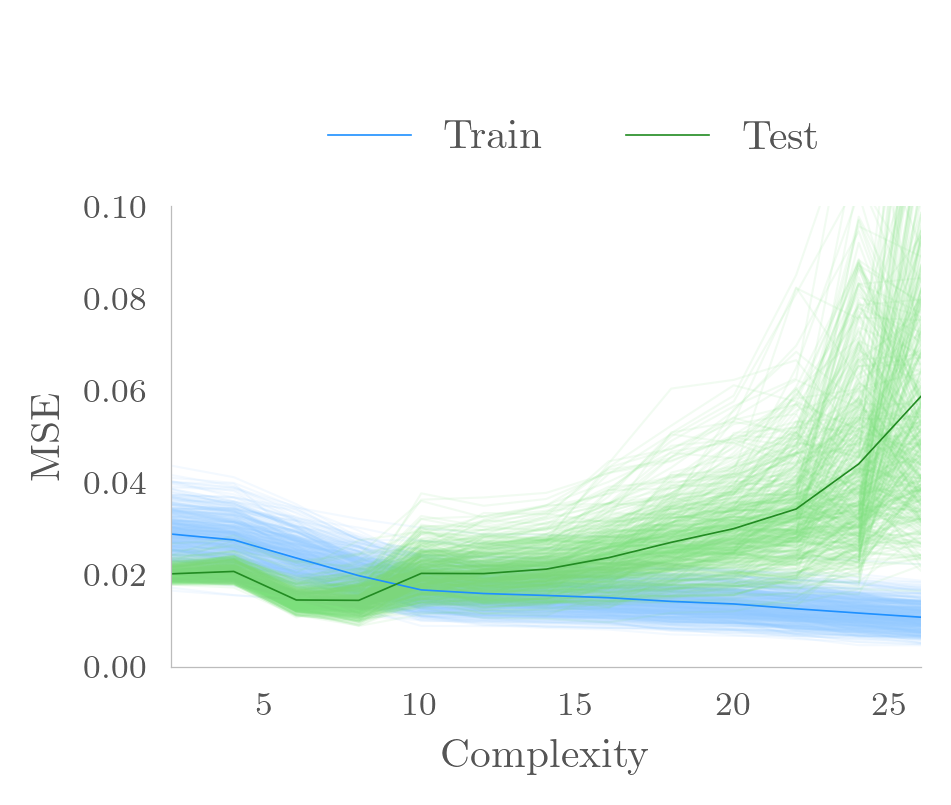
\includegraphics[]{figures/testrainmse.png}
  \caption{\label{fig:bias} Monte Carlo simulations run on the same data set
    with different random noise using OLS regression. The mean square error is
    computed for increasing model complexity. The Monte Carlo mean is shown in
    thicker lines and darker colors. The training MSE falls off
  to zero as the model complexity increases, while the test error initially
  decreases until the models begin to overfit the training set and the test
  error increases. Note also the spreading out of test variance as the complexity
  increases.} 
\end{figure}

\begin{figure}[]
  \centering
  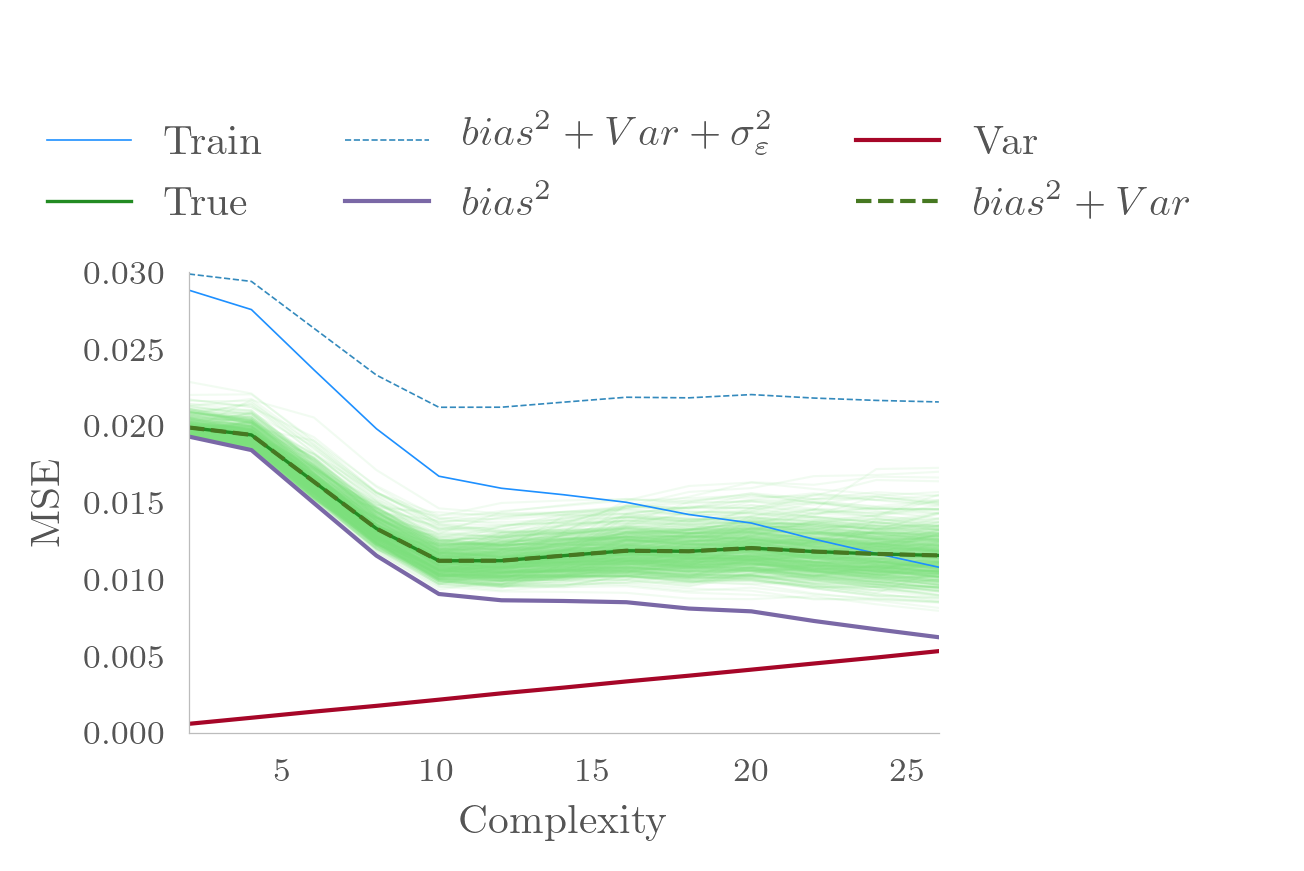
\includegraphics[]{figures/trainbiasvariance.png}
  \caption{\label{fig:biastrain} Same Monte Carlo simulation as~\cref{fig:bias}
  but showing the decomposition of the training error. The green lines show the
  Monte Carlo simulations of the training error minus the random noise. When the
squared bias is added to the variance, the sum is exactly as the mean of the
Monte Carlo simulations. As the random error is unknown, the actual training MSE
lies slighty higher. The bias decreases as the model complexity increases as the
model is better to explain the variance. However, as the model fits the training
error better and better, the variance increases.}
\end{figure}


\begin{figure}[]
  \centering
  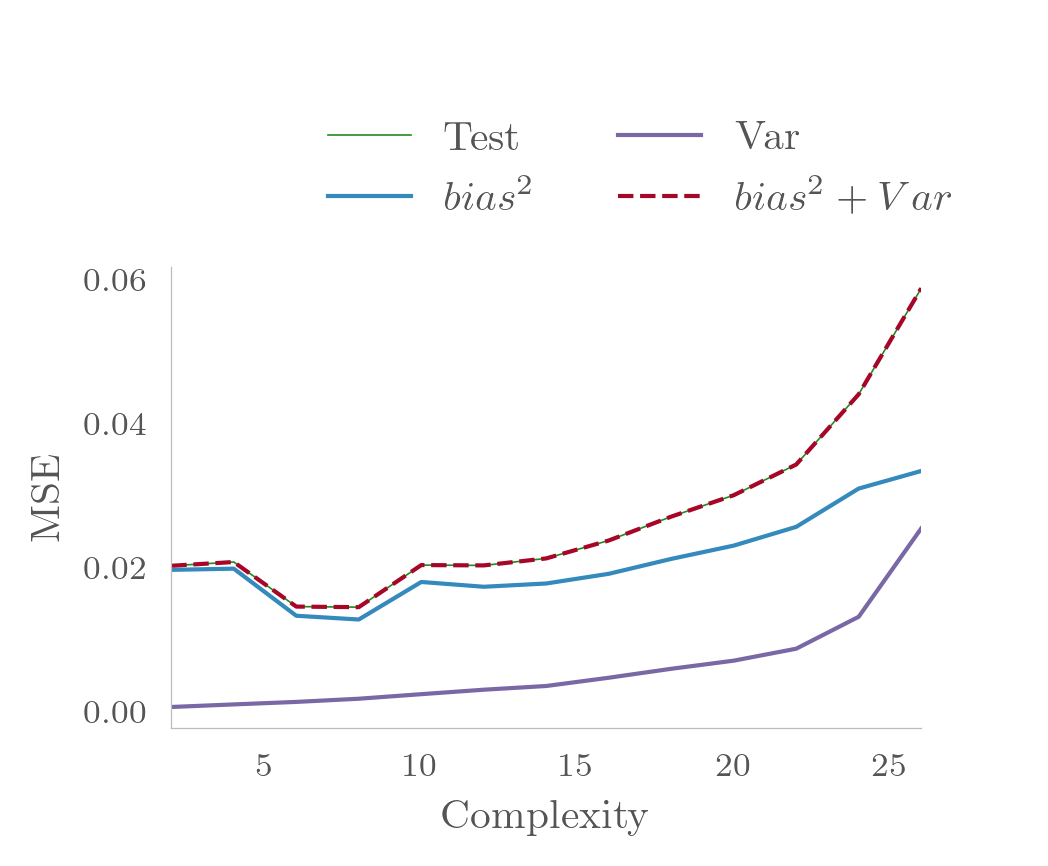
\includegraphics[]{figures/testbiasvariance.png}
  \caption{\label{fig:biastest} The same bias-variance decomposition as
    in~\cref{fig:biastrain} but on the test MSE. Adding the square bias to the
    variance matches the Monte Carlo mean of test MSE exactly. In difference to
    the training decomposition, the test bias increases after an initial
    decrease, the tell-tell sign of overfitting, and the variance increases
    faster at high complexity.}
\end{figure}
\subsection{Cross Validation}
\label{sec:cv}

When creating a model on a data set, it is necesarry to split the data up
into one training set and one test set for reasons outlined above. One often
uses a \(80\% - 20\%\) split. However, for small data sets it becomes infeasible
to both train and test a model with any reliability.

The solution is to use \textit{cross validation}, in particular \textit{k-fold}
cross validation. The data set is randomly shuffled and split into \(k\) folds.
Training takes place on \(k-1\) parts of the data while the remaining
\(k^{\text{th}}\) part is used for testing. This is repeated for \(k\) times,
giving \(k\) different estimates of the model coefficients and test error.

The cross validation estimate of the prediction error is CITE

\begin{equation*}
  \text{CV}(\hat f) = \frac{1}{N}\sum_{i=1}^{N}MSE(y_{i}, \hat f^{-\kappa(i)}(x_{i}))
\end{equation*}

where \(\hat f^{\kappa(i)}\) denotes the model fit with the \(k^{\text{th}}\)
part of the model removed.

Usual values for \(k\) is \(5\) or \(10\). For the rest of the paper, we will
only use \(k=5\) and usually samples of \(100\) observations. 

When selecting the best model, we use the ``one standard error'' rule where the
simplest model within one standard error of the best model is chosen. As the
``best'' model is not significantly better than the simpler model, this rule
errs on the side of accuracy for the sake of simplicity. 

